\documentclass[12pt,twoside]{article}
\usepackage{light}

%\hidesolutions
\showsolutions

\begin{document}

\problemset{9}{October 31, 2006}{\textit{Monday November 6 at 8 PM}}

\insolutions{}

\begin{problem}[15 points]

\bparts

\ppart Describe a bijection between the sequences $x_1,x_2, \dots, x_k$ of
positive integers such that
\begin{equation}\label{x1}
x_1 < x_2 < \cdots < x_k \leq n
\end{equation}
and the length $n$ bit-strings (i.e., strings of $\mathtt{0}$'s and
$\mathtt{1}$'s) containing exactly $k$ $\mathtt{1}$'s.

\solution{Map $(x_1,x_2, \dots, x_k)$ to
\[
\mathtt{0}^{x_1 - 1}\mathtt{1}
\mathtt{0}^{x_2 - x_1 - 1}\mathtt{1}
\mathtt{0}^{x_3 - x_2 - 1}\mathtt{1}\mathtt{0} \dots \mathtt{1}
\mathtt{0}^{x_k - x_{k - 1} - 1}\mathtt{1}
\mathtt{0}^{n-x_k}.
\]

Notice that there are exactly $k$ $\mathtt{1}$'s in the final string.
Also, the prefix of the string ending with $i$th $\mathtt{1}$ is exactly
$x_i$ letters long.  So the length of the prefix ending with the last
$\mathtt{1}$ is $x_k$, and the final string of $\mathtt{0}$'s ensures the
length of the whole string is $n$.

It's not hard to see how to recover the sequence from the bit-string it maps
to.  Also, we can recover a sequence from \emph{any} length $n$ bit-string
with $k$ \texttt{1}'s.  This means that the mapping from sequences to
bit-strings has an inverse mapping bit-strings back to sequences, which
implies that the mapping is indeed a bijection.

\medskip
Another, indirect, way to obtain a bijection is to observe that there is
bijection between the sequences satisfying~\eqref{x1} and the $k$-element
subsets of $\set{1,\dots,n}$.  Namely, map the sequence $(x_1,x_2, \dots,
x_k)$ to $\set{x_1,x_2, \dots, x_k}$.  We know there is a bijection
between these $k$-element subsets and bit-strings of length $n$ with $k$
occurrences of \texttt{1}'s.  Composing these two bijections yields a
bijection from sequences to bit-strings.}

\ppart Use the bijection to write a closed form (which may involve
factorials) for the number of sequences satisfying~\eqref{x1}.

\solution{
\[
\frac{n!}{k!(n-k)!} = \binom{n}{k}.
\]
}

\eparts

\end{problem}


\begin{problem}[20 points]
Every Halloween, 3 children visit your neighborhood
trick-or-treating. This year, you have 4 pieces of candy to give
them, all of which you will place into 3 bags. You can choose any
placement of candy in the bags, including leaving a bag empty (poor
kid!). How many placements are there if:

\bparts

\ppart You have 4 different types of candy, and the bags are labeled
for the children, Ann, Bob, and Cuauhtemoc?

\textit{Note:} once the pieces of candy are in a bag, there is no
way to tell the order in which they were placed.

\solution{ The answer is $81$.  We have $3$ choices for the first
piece of candy, $3$ choices for the second piece, etc.  The product
rule shows that there are $3^4 = 81$ ways in total. }

\ppart \label{2b} You only have 1 type of candy, and the bags are
unlabeled because you couldn't figure out how to spell ``Ann''
properly (i.e. the bags are indistinguishable except for the number
of pieces of candy in them)?

\solution{The answer is $4$.  there are four possibilities for the
number of pieces of candy in the bags: all 4 pieces in one bag; 3 in
one bag and 1 in another; 2 in one bag and 2 in another; or 2 in one
and 1 in each of the other two.  We do not care which pieces of
candy end up in which bag, so the number of ways is just $4$.}

\ppart You have 4 types of candy, but the bags are unlabeled?

\solution{The answer is $14$. As observed in part~(\ref{2b}), there
are four possibilities for the number of piece of candy in the bags:
all 4 pieces in one bag; 3 in one bag and 1 in another; 2 in one bag
and 2 in another; or 2 in one and 1 in each of the other two.  Since
the bags are not distinguishable, there is only one way to put all 4
pieces into the same bag.  Since the pieces \emph{are}
distinguishable, there are $\binom{4}{3}$ ways of putting 3 pieces
into one bag, and this determines which ball is by itself in the
other non-empty bag. There are $\binom{4}{2}/2$ of putting 2 pieces
in one bag and 2 in another.  There are $\binom{4}{2}$ ways of
putting 2 in one and 1 in each of the other two.  So the total
number of ways is
\[
1 + \binom{4}{3} + \frac{1}{2}\binom{4}{2} + \binom{4}{2} = 14.
\]}

\ppart The bags are labeled, but you only have 1 type of candy?

\solution{The answer is $15$.  This is like the problem of choosing
a dozen donuts seen in lecture.  Here the bags are the ``types of
donuts'' and the pieces correspond to the donuts whose type we can
choose.  (This sort of problem is also known as a ``stars and bars''
problem: the donuts are the stars, and the bars are the separators
between the types of donuts.)  The answer is
\[
\binom{4+3-1}{4} = \binom{6}{4} = 15.
\]}

\eparts

\end{problem}


\begin{problem}[15 points]
An urn contains balls numbered from 1 to 9. You draw 6 balls from
the urn. How many different \emph{ordered} draws can you get if:

\bparts

\ppart Ball 1 is included in the draw?

\solution{There are $6$ ways to choose the position of ball 1 in the
ordering, and $8 \cdot 7 \cdot 6 \cdot 5 \cdot 4$ ways to choose and
arrange the others. So the total is:
\[
6 \cdot \frac{8!}{3!} = 40320.
\]
}

\ppart Ball 1 and ball 2 are both included in the draw?

\solution{There are $6$ ways to place ball 1 and $5$ ways to place
ball 2. There are $7 \cdot 6 \cdot 5 \cdot 4$ ways to choose and
arrange the others. So the total is:
\[
6 \cdot 5 \cdot \frac{7!}{3!} = 25200.
\]}


\ppart Exactly one of ball 1 and ball 2 is included in the draw?

\solution{There are $2$ ways to choose between ball 1 and ball 2,
$6$ ways to place whichever one is chosen, and $7 \cdot 6 \cdot 5
\cdot 4 \cdot 3$ to choose and arrange the remaining people.  Total:
$$2 \cdot 6 \cdot \frac{7!}{2!} = 6 \cdot 7! = 30240.$$}

\eparts

\end{problem}


\instatements{\newpage}

\begin{problem}[10 points]
(The two parts of this problem are independent.)

\bparts

\ppart Describe a bijection between the length $n$ bit-strings with an
even number of \texttt{1}'s and the length $n$ bit-strings with an odd
number of \texttt{1}'s.  Explain why any such bijection leads to a simple
formula for the number of even-size subsets of any set of size $n$.

\solution{
Map a string to the same string with the first bit complemented.  This map
is its own inverse, and hence is a bijection from length $n$ bit-strings to
length $n$ bit-strings.  Restricting it to the length $n$ bit-strings with
an even number of \texttt{1}'s yields a bijection between the length $n$
bit-strings with an even number of \texttt{1}'s and the length $n$
bit-strings with an odd number of \texttt{1}'s.  So there are the same
number of strings of each kind, and therefore exactly half of the length
$n$ bit-strings have an even number of \texttt{1}'s, namely, $2^n/2 =
2^{n-1}$ strings with an an even number of \texttt{1}'s.

But with the standard bijection between bit-strings of length $n$ and
subsets of a set of size $n$, the strings with an even number of
\texttt{1}'s correspond to even-size subsets.  So the number of even-size
subsets is also $2^{n-1}$.
}

\ppart A shelf holds 12 books in a row.  How many ways are there to choose
five books so that no two adjacent books are chosen?

\solution{There are 5 bars (chosen books), and therefore there are 6
places where the 7 stars (non-chosen books) can fit (before the first bar,
between the first and second bars,..., after the fifth bar).  Each of the
second through fifth of these slots must have at least one star in it, so
that adjacent books are not chosen. Once we have placed these 4 stars,
there are 3 stars left to be placed in 6 slots. The number of ways to do
this is therefore
\[
\binom{6+3-1}{3}=\binom{8}{3}=56.
\]}


\eparts

\end{problem}

%new for F04, variant of old Karger problem

\begin{problem}[15 points]
Suppose we have $n$ distinct points on the sphere, where the sphere is taken to mean all points of the form $(x,y,z) \in \mathcal{R}^3$ with $x^2 + y^2 + z^2 = 1$. Show that there is a closed hemisphere containing $2 + \lceil \frac{n-2}{2} \rceil$ of the $n$ points. 

Here, by closed hemisphere we mean exactly half of the sphere, including its boundary points. For instance, if we take two distinct points $p,q$ on the sphere, and draw the unique circle $C$ containing $p$ and $q$ centered at the origin, then the sphere decomposes into two closed hemispheres with common intersection $C$.

\solution{
Consider any $2$ of the $n$ points, say $p$ and $q$, and draw the circle $C$ containing $p$ and $q$ centered at the origin. This divides the sphere into two closed hemispheres with common intersection $C$. By the pigeonhole principle, $\lceil \frac{n-2}{2} \rceil$ of the remaining points must lie in one of the hemispheres, and since the hemisphere is closed, there are $2 + \lceil \frac{n-2}{2} \rceil$ points in that hemisphere.
}

\end{problem}

%minor variant of spring01 tut8 & tutorial 9, spring 00.
       % Uses division rule.

\begin{problem}[15 points]
We want to split the class into teams of four.  Suppose there are $4n$
students in the class, so there should be $n$ teams.  Write a simple
closed-form formula (which may involve factorials) for the number of ways
the class could be split.  Explain your answer.

\solution{
\begin{equation}\label{3nf}
\frac{(4n)!}{n! \cdot 24^n}
\end{equation}

There are $(4n)!$ sequences consisting of the distinct students.  From
such a sequence, we can split into teams by teaming up the first four
students, the next four students, \dots, the last four students.

Now we observe that for a given split, there are $n!$ sequences of
\emph{teams} that describe that split.  Each team can be ordered in $4!$
ways, so there are $(4!)^n$ ways to order every one of the teams.  That
is, each split arises from exactly $n! \cdot 24^n$ sequences.
So~\eqref{3nf} follows by the Division Rule.}
\end{problem}

%%%%%%%%%%%%%%%%%%%%%%%%%%%%%%%%%%%%%%%%%%%%%%%%%%%%%%%%%%%%%%%%%%%%%%%%%%%%

\begin{problem}[10 points]
In preparation for a 6.042 study session, you want to calculate the
number of different ways to make sundaes for you and your friends.
You have 10 different toppings, and you want to make four sundaes
such that each sundae has between one and four (inclusive) toppings,
and you don't reuse any toppings. The sundaes are going to 4
different people, so their order matters! How many ways can this be
done?

\solution{We first enumerate the different ways to divide up 10
toppings to the 4 sundaes, where we don't distinguish between
toppings, and the order of the sundaes doesn't matter. One such way
would be to put 1 topping on one sundae, and 3 on each of the other
3, denoted by $[1, 3, 3, 3]$. Similarly, we have $[1, 1, 4,
4]$, $[1, 2, 3, 4]$, $[2, 2, 3, 3]$, and $[2, 2, 2, 4]$.\\

Now, let's consider the order of the sundaes. For $[1, 3, 3, 3]$, we
also have [3, 1, 3, 3], [3, 3, 1, 3], and [3, 3, 3, 1], so there are
4 ways to get 1 topping on 1 sundae and 3 on each of the other 3
(also, $4!/3!$, as we have 4 elements to order, 3 of which are the
same). Similarly, we have $4!/(2!2!) = 6$ ways of getting $[1, 1, 4,
4]$, $4! = 24$ ways for $[1, 2, 3, 4]$, $4!/(2!2!) = 6$ ways for
$[2, 2, 3, 3]$, and $4!/3! = 4$ ways for $[2, 2, 2, 4]$.\\

Finally, let's distinguish between the toppings. We assume that the
order of toppings on a given sundae doesn't matter (i.e. a sundae
with fudge and whipped cream is the same as a sundae with whipped
cream and fudge). We then have $10!/(1!3!3!3!)$ ways to distinguish
between toppings when we have the division $[1, 3, 3, 3]$, and so
on. Therefore, the final answer is:

$$
4\frac{10!}{1!3!3!3!} + 6\frac{10!}{1!1!4!4!} +
24\frac{10!}{1!2!3!4!} + 6\frac{10!}{2!2!3!3!} +
4\frac{10!}{2!2!2!4!}
$$
$$
= 10!(\frac{4}{216} + \frac{6}{576} + \frac{24}{288} + \frac{6}{144}
+ \frac{4}{192}) = 634200.
$$

(Note that this is a large proportion of the total $4^{10} =
1048576$ ways to distribute 10 toppings to 4 sundaes, so our
restrictions weren't that restrictive!)


}

%\solution{First put one topping on each sundae. Then we must
%distribute six toppings on four sundaes in such a way that no more
%than three toppings are on the same sundae.  We use
%inclusion/exclusion.
%
%Number of ways to place six toppings on 4 sundaes is
%\[
%\binom{6+4-1}{6} = \binom{9}{6}.
%\]
%
%Number of ways to place six toppings on 4 sundaes such that there
%are four toppings on a sundae = number of ways to choose a sundae
%with three toppings $\times$ number of ways to place two toppings on
%three sundaes =
%\[
%4 \cdot \binom{4}{2}.
%\]
%
%Number of ways to place six toppings on 4 sundaes such that there
%are five toppings on a sundae =
%\[
%4 \cdot \binom{3}{1}.
%\]
%
%Number of ways to place six toppings on 4 sundaes such that there
%are six toppings on a sundae = $4$.
%
%So the total number of ways is
%\[
%\binom{9}{6} - 4 \cdot \binom{4}{2} - 4 \cdot \binom{3}{1} - 4 = 44.
%\]
%}

\end{problem}


\iffalse
%%REUSED FROM Fall02 cp8W

\begin{problem}[20 points]
A \emph{numbered tree} is a tree whose vertex set is
$\set{1,2,\dots,n}$ for some $n \geq 2$.  We define the \emph{code} of
the numbered tree to be a sequence of $n-2$ integers from 1 to $n$
obtained by the following recursive process:
\begin{quotation}
If $n=2$, stop---the code is the empty sequence.  Otherwise, write down
the \emph{father} of the largest leaf, delete this \emph{leaf}, and
continue the process on the resulting smaller tree.
\end{quotation}

For example, the codes of a couple of numbered trees are shown in
the Figure~\ref{codetrees}.

\begin{figure}[htb]
\begin{center}
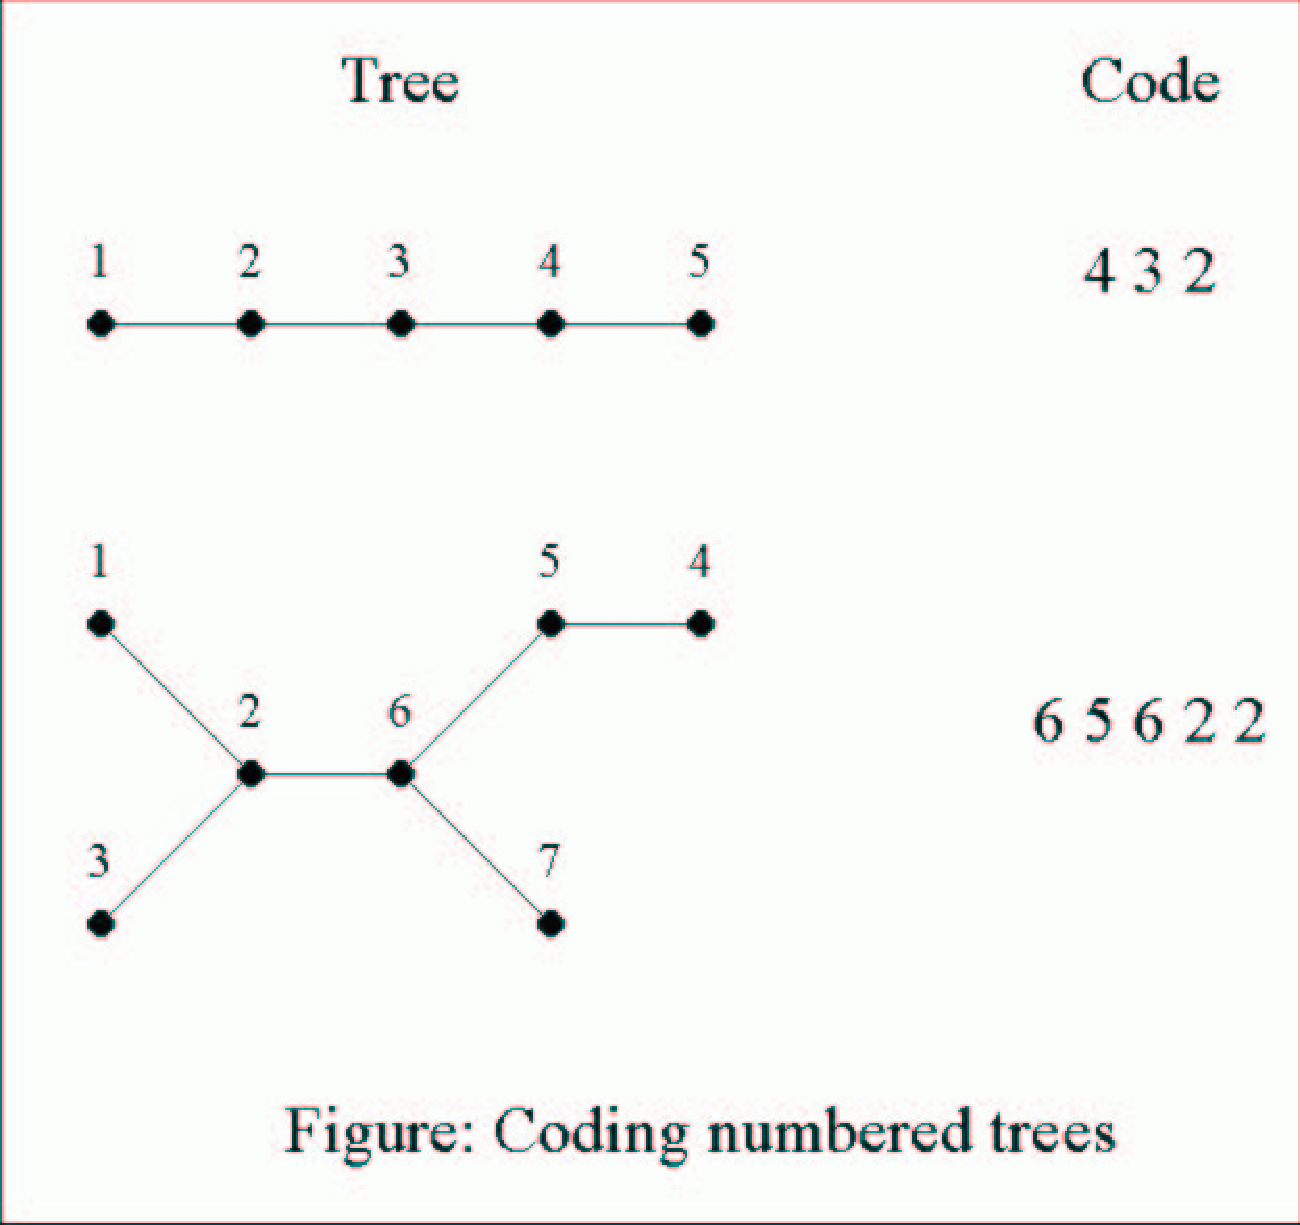
\includegraphics[width=4in]{figures/n-2}
\end{center}
\caption{}
\label{codetrees}
\end{figure}

\bparts

\ppart Describe a procedure for reconstructing a numbered tree from
its code.

\solution{
The key observation is that, given a code of length $n-2$, the numbers
between 1 and $n$ which \emph{do not appear} in the code must be leaves of
the tree.  Hence, the largest missing number is a leaf attached to the
first number of the code.  The rest of the tree can now be reconstructed
by deleting the first number in the code, henceforth ignoring the largest
leaf, and proceeding recursively on the rest of the code.  (We're using
the obvious fact that what's left after deleting a leaf from a tree is
another tree.)

More precisely, the reconstruction procedure applies to any finite tree
whose vertex set is totally ordered.  The procedure takes \emph{two}
parameters: the vertex set, $V$, and a length $\size{V}-2$ ``code''
sequence, $S$, of elements in $V$.  If $l$ is the largest element in $V$
which does not appear in $S$, and $f$ is the first element of $S$, then
the reconstructed tree is obtained by adding edge $(l,f)$ to the tree
reconstructed by calling the procedure recursively with first argument
$V-\set{l}$ and second argument equal to the code obtained by erasing the
initial $f$ from $S$.  The procedure terminates when $\size{V}=2$,
returning the edge between the two numbers in $V$.

%This paragraph is correct, but would benefit from a rewrite:

To justify the key observation, note that any vertex that gets deleted by
the process and was not a leaf to begin with, must have been the father of
a previously deleted leaf, which means it would appear in the code.  So
the missing integers must have been leaves to begin with or must be one of
the two undeleted vertices left when the coding process terminates.  But
by the end of the process the two remaining vertices are leaves, and if
they weren't leaves to begin with, they must have become leaves by having
their sons deleted, which means they would not have been missing from the
code.  So the two vertices remaining at the end must also have been leaves
of the original tree.
}

\ppart How many numbered trees with $n$ vertices are there?  Justify
your answer assuming the result of the previous problem part.

\solution{There are exactly as many $n$-vertex numbered trees as the
number of possible code words, that is, the number of length $n-2$
sequences integers between 1 and $n$.  So there are $n^{n-2}$ numbered
trees.

The reason is that the map from trees to codes is a bijection.  To see
this, note that the tree reconstruction procedure finds \emph{the only
possible tree} with that code.  So there can't be two trees with the same
code, i.e., the map from a tree to its code is an injection.  But since
the reconstruction procedure finds a tree for every possible codeword, the
map from trees to codes is also a surjection.}

\eparts
\end{problem}
\fi


\end{document}
